\section{FitzHugh-Nagumoモデル}
\subsection{FitzHugh-Nagumoモデルの定義}

前節では神経活動のダイナミクスを微分方程式で表したHodgkin-Huxley(HH)モデルを扱った.HHモデルの特徴は,4変数で構成され,各変数が膜電位およびNaチャネルやKチャネルなどの活性/不活性状態を意味することである.このHHモデルをより簡易化し,2変数で神経活動の興奮とその伝播を表そうと提案されたのが\textbf{FitzHugh-Nagumo (FHN)モデル}\index{FitzHugh-Nagumo (FHN)もでる@FitzHugh-Nagumo (FHN)モデル} である.FHNモデルはvan der Pol振動子をFitzHughが修正し\citep{FitzHugh1955-bx} \citep{Fitzhugh1961-fp},南雲らによりトンネル (江崎) ダイオードを用いて電子回路上に実装\footnote{神経活動を再現する電子回路を\textbf{ニューリスタ}\index{にゅーりすた@ニューリスタ}  (neuristor) という.}された \citep{Nagumo1962-ob}という経緯がある.FHNモデルは以下で表される.


\begin{align} 
\frac{dv}{dt} &= c\left(v-\frac{v^3}{3}-u+I_e\right)\\ 
\frac{du}{dt} &= v-bu+a 
\end{align}


$v$は膜電位で,$u$は回復変数(recovery variable)と呼ばれる. FitzHughにより,HHモデルにおける$(V, m)$および$(n, h)$がそれぞれFHNモデルの$v$および$u$に対応すると説明されている \citep{Fitzhugh1961-fp} \footnote{HHモデルにおける$V$と$m$は強い正の相関があり,$n$と$h$は強い負の相関があるため,それぞれの変数の組は1つの変数に縮約されうる.}.$a,b,c$は定数であり,$a=0.7, b=0.8, c=10$がよく使われる.$I_e$は外部刺激電流に対応する.
\lstinputlisting[language=julia]{./text/neuron-model/fhn/001.jl}
変更しない定数を保持する \jl{struct} の \jl{FHNParameter} と, 変数を保持する \jl{mutable struct} の \jl{FHN} を作成する.
\lstinputlisting[language=julia]{./text/neuron-model/fhn/003.jl}
次に変数を更新する関数\jl{update!}を書く.ソルバーとしては陽的Euler法または4次のRunge-Kutta法を用いる.以下ではEuler法を用いている.Juliaではforループを用いて1つのニューロンごとにパラメータを更新する方がベクトルを用いるよりも高速である.
\lstinputlisting[language=julia]{./text/neuron-model/fhn/005.jl}
\subsection{FitzHugh-Nagumoモデルのシミュレーションの実行}
いくつかの定数を設定してシミュレーションを実行する.
\lstinputlisting[language=julia]{./text/neuron-model/fhn/007.jl}
結果を描画する.
\lstinputlisting[language=julia]{./text/neuron-model/fhn/009.jl}
\begin{figure}[ht]
	\centering
	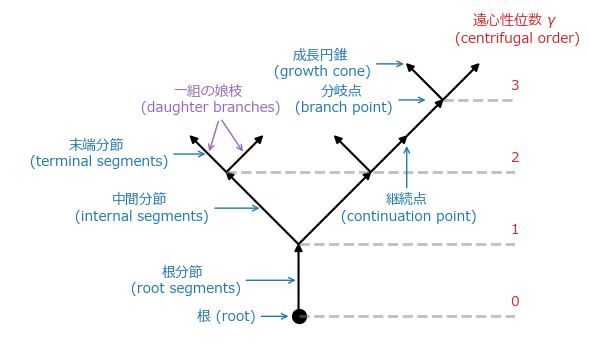
\includegraphics[scale=0.8, max width=\linewidth]{./fig/neuron-model/neurite-growth-model/cell009.png}
	\caption{cell009.png}
	\label{cell009.png}
\end{figure}
\subsection{相図の描画}
phase plot
\lstinputlisting[language=julia]{./text/neuron-model/fhn/011.jl}
\lstinputlisting[language=julia]{./text/neuron-model/fhn/012.jl}
\begin{figure}[ht]
	\centering
	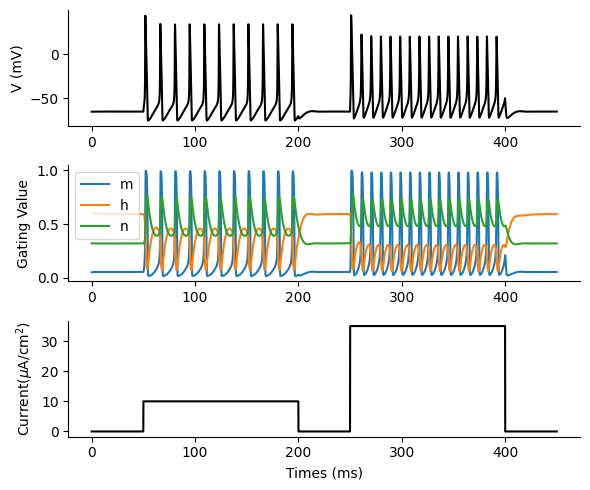
\includegraphics[scale=0.8, max width=\linewidth]{./fig/neuron-model/hodgkin-huxley/cell012.png}
	\caption{cell012.png}
	\label{cell012.png}
\end{figure}
